\documentclass{easychair}

% \usepackage{doc}
\usepackage{setspace}
\usepackage{verbatim}
\usepackage{wasysym}

%----Making things more compact
\newcommand{\smalltt}[1]{\small \texttt{#1}}
\newenvironment{packed_itemize}{
\vspace*{-0.2em}
\begin{itemize}
\setlength{\partopsep}{0pt}
\setlength{\itemsep}{1pt}
\setlength{\parskip}{0pt}
\setlength{\parsep}{0pt}
}{\end{itemize}}
\newenvironment{packed_enumerate}{
\vspace*{-0.2em}
\begin{enumerate}
\setlength{\partopsep}{0pt}
\setlength{\itemsep}{1pt}
\setlength{\parskip}{0pt}
\setlength{\parsep}{0pt}
}{\end{enumerate}}
% \renewcommand{\textfraction}{0.07}
% \renewcommand{\topfraction}{0.9}
% \renewcommand{\bottomfraction}{0.9}
% \renewcommand{\floatpagefraction}{0.66}
% \setlength{\floatsep}{2.0pt plus 2.0pt minus 2.0pt}
% \setlength{\textfloatsep}{5.0pt plus 2.0pt minus 0.0pt}

\title{Stepping Stones in the TPTP World}

\author{
  Geoff Sutcliffe
}

\institute{
  University of Miami,
  Miami, USA\\
  \email{geoff@cs.miami.edu}\\
}

\authorrunning{Geoff Sutcliffe}
\titlerunning{Stepping Stones in the TPTP World}

\begin{document}
\maketitle

%--------------------------------------------------------------------------------------------------
\begin{abstract}
The TPTP World is a well established infrastructure that supports research, development, and 
deployment of Automated Theorem Proving (ATP) systems.
There have been some key developments that helped make the TPTP World a success: 
the TPTP problem library was first released in 1993,
the CADE ATP System Competition (CASC) was conceived after CADE-12 in Nancy in 1994, 
problem difficulty ratings were added in 1997, 
the current TPTP language was adopted in 2003, 
the SZS ontologies were specified in 2004, 
the TSTP solution library was built starting around 2005, 
the Specialist Problem Classes (SPCs) have been used to classify problems from 2010, 
the SystemOnTPTP service has been offered from 2011, 
the StarExec service was started in 2013,
and 
a world of TPTP users have helped all along.
This paper reviews these stepping stones in the development of the TPTP World.
\end{abstract}
%--------------------------------------------------------------------------------------------------
\section{Introduction}
\label{Introduction}

The TPTP World~\cite{Sut10,Sut17} (once gently referred to as the ``TPTP Jungle''~\cite{BU13}) is 
a well established infrastructure that supports research, development, and deployment of 
Automated Theorem Proving (ATP) systems.
Salient components of the TPTP World are
the TPTP problem library~\cite{Sut09}, 
the TSTP solution library~\cite{Sut10}, 
the TPTP languages~\cite{SS+06}, 
the SZS ontologies~\cite{Sut08-KEAPPA},
the Specialist Problem Classes (SPCs) and problem difficulty ratings~\cite{SS01},
and the CADE ATP System Competition (CASC)~\cite{Sut16}.
SystemOnTPTP~\cite{Sut00-CADE-17} and StarExec~\cite{SST14} provide computational support for
the TPTP World.
There are dependencies between these parts of the TPTP World, as shown in 
Figure~\ref{Dependencies}, forming a series of "stepping stones" from TPTP standards to 
happy users~\ldots
\begin{packed_itemize}
\item The TPTP language (see Section~\ref{Languages}) is used for writing problems in the TPTP
      problem library and the TSTP solution library.
\item The SZS ontologies (see Section~\ref{SZS}) are used to specify properties of problems
      and solutions.
\item The SPCs (see Section~\ref{SPCs}) that classify problems are based on the language form 
      and SZS ontology values.
\item The TPTP problem library (see Section~\ref{TPTP}) is the central collection of test problems.
\item The TSTP solution library (see Section~\ref{TSTP}) is the central collection of solutions
      to the TPTP library problems.
\item The TPTP problems' difficulty ratings (see Section~\ref{Ratings}) are computed wrt each
      SPC, using data from the TSTP.
\item The CADE ATP System Competition (see Section~\ref{CASC}) is the annual evaluation of 
      ATP systems - the world championship for such systems.
\item SystemOnTPTP (see Section~\ref{StarExec}) provides online access to ATP systems and tools.
\item The StarExec computers (see Section~\ref{StarExec}) are used to build the TSTP, and to run
      CASC.
\item Users of the TPTP World (see Section~\ref{Users}) provide problems for the TPTP problem
      library, and ATP systems/tools for SystemOnTPTP and StarExec.
\end{packed_itemize}
There is a cycle of dependencies from the TPTP problem library, to the TSTP solution 
library, to the problem difficulty ratings, and back to the TPTP problem library.
This cycle means that building these components, particularly building releases of the TPTP 
problem library, requires iteration until stability is reached.

\begin{figure}[htbp]
\centering
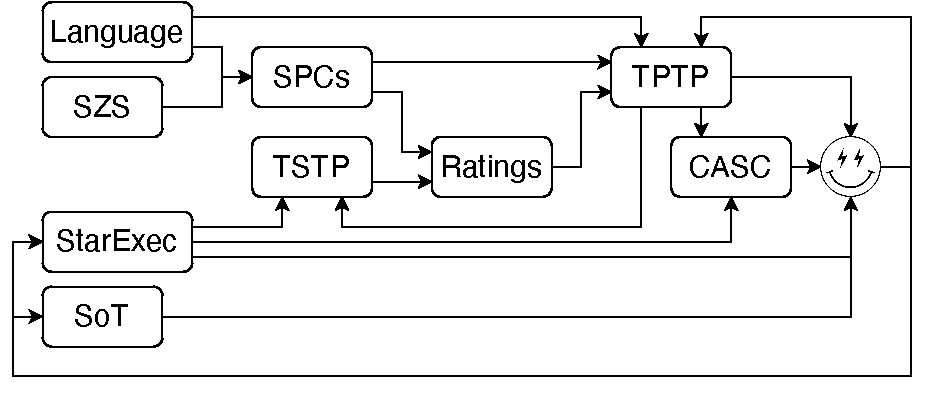
\includegraphics[width=0.75\textwidth]{Dependencies.pdf}
\caption{Dependencies between the Stepping Stones}
\label{Dependencies}
\end{figure}

Various parts of the TPTP World have been deployed in a range of applications, in both academia 
and industry.
Since the first release of the TPTP problem library in 1993, many researchers have used the 
TPTP World as an appropriate and convenient basis for ATP system research and development. 
The web page \href{http://www.tptp.org}{{\tt www.tptp.org}} provides access to all components.

\paragraph{This paper is organized as follows:}

%--------------------------------------------------------------------------------------------------
\section{The TPTP Languages}
\label{Languages}

The TPTP language~\cite{Sut23-IGPL} is one of the keys to the success of the TPTP World.
The TPTP language is used for writing both problems and solutions,
which enables convenient communication between TPTP-compliant ATP systems and tools.
Originally the TPTP World supported only first-order clause normal form (CNF)
\cite{SS98-JAR}.
Over the years full first-order form (FOF)
\cite{Sut09}, 
typed first-order form (TFF)
\cite{SS+12,BP13-TFF1}, 
typed extended first-order form (TXF)
\cite{SK18}, 
typed higher-order form (THF)
\cite{SB10,KSR16}, 
and non-classical forms (NTF)~\cite{SF+22} have been added.
The standardisation of the language received a signifcant technical boost in 2006 when the BNF
definition was revised to a state that a parser could be automatically generated using
{\tt lex/yacc}~\cite{VS06}, and all the language forms are now quite precisely 
specified.\footnote{%
But note that the BNF ``syntax'' is not completely strict -- the BNF uses an extended BNF form
that relgates details to ``strict'' rules that do not have to be checked by a parser.}
A general principle of the TPTP language is ``we provide the syntax, you provide the semantics''.
As such, there is no a priori commitment to any semantics for the languages, although in almost 
all cases the intended logic and semantics are well known.

The formulae of problems solutions are built from {\em annotated formulae}, 
which have the form~\ldots \\
\hspace*{0.5cm}{\em language}{\tt (}{\em name}{\tt ,}
{\em role}{\tt ,}
{\em formula}{\tt ,}
{\em source}{\tt ,}
{\em useful\_info}{\tt )}\\
The {\em language}s supported are {\smalltt{cnf}} (clause normal form), {\smalltt{fof}}
(first-order form), {\smalltt{tff}} (typed first-order form), and {\smalltt{thf}}
(typed higher-order form).
The {\em role}, e.g., {\smalltt{axiom}}, {\smalltt{lemma}}, {\smalltt{conjecture}}, defines the 
use of the formula in an ATP system.
In a {\em formula}, terms and atoms follow Prolog conventions -- functions and predicates start 
with a lowercase letter or are {\tt '}single quoted{\tt '}, and variables start with an uppercase 
letter.
The language also supports interpreted symbols that either start with a {\tt \$}, e.g., the 
truth constants {\smalltt{\$true}} and {\smalltt{\$false}}, or are composed of 
non-alphabetic characters, e.g., integer/rational/real numbers such as 27, 43/92, -99.66.
The logical connectives in the TPTP language are
{\tt !}, {\tt ?}, {\tt {\raisebox{0.4ex}{\texttildelow}}}, {\tt |}, {\tt \&}, {\tt =>}, {\tt <=},
{\tt <=>}, and {\tt <{\raisebox{0.4ex}{\texttildelow}}>},
for the mathematical connectives
$\forall$, $\exists$, $\neg$, $\vee$, $\wedge$, $\Rightarrow$, $\Leftarrow$, $\Leftrightarrow$, 
and $\oplus$ respectively.
Equality and inequality are expressed as the infix operators {\tt =} and {\tt !=}.
The {\em source} and {\em useful\_info} are optional.
Figure~\ref{ExampleFormulae} shows an example with typed higher-order annotated formulae.

\begin{figure}[htb]
{\footnotesize
{\setlength{\baselineskip}{3mm}
\begin{verbatim}
%------------------------------------------------------------------------------
thf(beverage_decl,type,   beverage: $tType ).
thf(syrup_decl,type,      syrup: $tType ).
thf(coffee_type,type,     coffee: beverage ).
thf(mix_type,type,        mix: beverage > syrup > beverage ).
thf(heat_type,type,       heat: beverage > beverage ).
thf(heated_mix_type,type, heated_mix: beverage > syrup > beverage ).
thf(hot_type,type,        hot: beverage > $o ).

thf(heated_mix,axiom,
    ( heated_mix
    = ( ^ [B: beverage,S: syrup] : ( heat @ ( mix @ B @ S ) ) ) ) ).

thf(hot_mixture,axiom,
    ! [B: beverage,S: syrup] : ( hot @ ( heated_mix @ B @ S ) ) ).

thf(heated_coffee_mix,axiom,
    ! [S: syrup] : ( ( heated_mix @ coffee @ S ) = coffee ) ).

thf(hot_coffee,conjecture,
    ? [Mixture: syrup > beverage] :
    ! [S: syrup] :
      ( ( ( Mixture @ S ) = coffee )
      & ( hot @ ( Mixture @ S ) ) ) ).
%------------------------------------------------------------------------------
\end{verbatim}
}}
\caption{THF annotated formulae}
\label{ExampleFormulae}
\end{figure}

%--------------------------------------------------------------------------------------------------
\section{The TPTP Problem Library}
\label{TPTP}

The first inklings of the TPTP World were at CADE-10 in Kaiserslautern, Germany, in 1990, as a 
collaboration between Geoff Sutcliffe at the University of Western Australia (James Cook 
University from 1993), and Christian Suttner at the Technische Universit{\"a}t M{\"u}nchen.
At that time a large number of interesting test problems had accumulated in the ATP community, in
both hardcopy~\cite{MOW76,WM76,Pel86-JAR,BL+86,Qua92-JAR,MW92-CADE-11} and electronic form
\cite{ANL,SPRFN}.\footnote{To my knowledge, the first circulation of test problems was by 
Larry Wos in the late sixties.} 
We observed that ATP system developers were testing their systems, and publishing results, 
based on small numbers of selected test problems.
At the same time some good ideas were seen to be abandoned because they had been tested on
inappropriate selections of test problems.
These observations motivated us to start collecting ATP test problems into what became the TPTP 
problem library.
The goal was to support testing and evaluation of ATP systems, to help ensure that performance 
results accurately reflect the capabilities of the ATP systems being considered. 
A common library of test problems is necessary for meaningful system evaluations, meaningful system 
comparisons, repeatability of testing, and the production of statistically significant results. 
The TPTP problem library was designed to centralize and unify these disparate collections, 
to provide a comprehensive library of ATP test problems in a simple, unambiguous, reference 
mechanism.
The first release of the TPTP problem library was made on Friday 12th November 1993. 

The TPTP problem library is managed in the manner of a software product, in the sense that fixed 
releases are made.
Each release is identified by a release number in the form v$Version$.$Edition$.$Patch$:
the $Version$ enumerates major new releases of the TPTP in which important new features have 
been added,
the $Edition$ is incremented each time new problems are added to the current version, and
the $Patch$ level is incremented each time errors found in the current edition are corrected. 

The problems in the library are classified into {\em domains} that reflect a natural hierarchy.
Seven main fields are defined: logic, mathematics, computer science, science \& engineering, 
social sciences, arts \& humanities, and other. 
Each field is subdivided into domains, each identified by a three-letter mnemonic, e.g., the
social science field has three domains: Social Choice Theory (SCT), Management (MGT), and
Geography (GEG).

Table~\ref{tab:Releases} lists the versions of the TPTP up to v9.0.0, with the new feature added, 
the number of problem domains, and the number of problems.\footnote{%
The data for v9.0.0 is an estimate, because this paper was written before the release was
finalised.}
The number of domains indicates the diversity of the problems, while the number of problems 
indicates the size of the library.
The attentive reader might note that many releases have been made in July/August.
This is because the CADE ATP System Competition (CASC - see Section~\ref{CASC}), has an 
influence on the release cycle of the TPTP. 

\begin{table}[htb]
\begin{center}
\setlength{\tabcolsep}{4pt}
\begin{tabular}{ll|l|rr}
Release & Date     & Changes                                              & Domains & Problems \\
\hline
v1.0.0  & 12/11/93 & First public release, only CNF~\cite{SS98-JAR}       &      23 &     2295 \\
v2.0.0  & 05/06/97 & FOF~\cite{Sut09} and ratings (Section~\ref{Ratings}) &      28 &     3277 \\
v3.0.0  & 11/11/04 & New TPTP language~\cite{SS+06}                       &      32 &     7267 \\
v4.0.0  & 04/07/09 & TH0 (monomorphic typed higher-order)~\cite{SB10}     &      41 &    16512 \\
v5.0.0  & 16/09/10 & TF0 (monomorphic typed first-order)~\cite{SS+12}     &      45 &    18480 \\
v6.0.0  & 21/09/13 & TF1 (polymophic typed first-order)~\cite{BP13-TFF1}  &      48 &    20306 \\
v7.0.0  & 24/07/17 & TH1 (polymophic typed higher-order)~\cite{KSR16}     &      53 &    21851 \\
v8.0.0  & 19/04/22 & TXF (typed extended first-order)~\cite{SK18}         &      54 &    24785 \\
v9.0.0  & ??/07/24 & NTF (non-classical typed first-order)~\cite{SF+22}   &      55 &    25598 \\
\end{tabular}
\end{center}
\caption{Overview of TPTP releases}
\label{tab:Releases}
\end{table}

% TPTP problem files present the logical formulae in a format that is both human and machine 
% readable, and additionally provide useful information for users.
% The file names are built from the domain acronym, a 3 digit problem number, a separator that
% indicates the syntax ({\tt -} for CNF, {\tt +} for FOF, {\tt \_} for TFF, {\tt \verb|^|} for THF),
% optional digits for the problem size, and a problem version number.
Each TPTP problem file has three parts: a header, optional includes, and annotated formulae.
The header section contains information for users, formatted as comments in four parts:
the first part identifies and describes the problem;
the second part provides information about occurrences of the problem
in the literature and elsewhere;
the third part provides semantic and syntactic characteristics of the problem;
the last part contains comments and bugfix information.
The include section is optional, and if used contains {\tt include} directives for axiom files,
which in turn have the same three-part format as problem files.
Their inclusion avoids the need for duplication of the formulae in commonly used axiomatizations.
The annotated formulae are described in Section~\ref{Languages}.
Figure~\ref{ExampleHeader} shows an example header and {\tt include} section.
The header fields are self-explanatory, but of particular interest are the {\tt Status} field 
that is explained in Section~\ref{SZS}, the {\tt Rating} field that is explained in 
Section~\ref{Ratings}, and the {\tt SPC} field that is explained in Section~\ref{SPCs}.

\begin{figure}[htb]
{\footnotesize
{\setlength{\baselineskip}{3mm}
\begin{verbatim}
%------------------------------------------------------------------------------
% File     : DAT016_1 : TPTP v8.2.0. Bugfixed v5.1.0.
% Domain   : Data Structures
% Problem  : Some element is 53
% Version  : [PW06] axioms.
% English  : Show that some element of the array has the value 53.

% Refs     : [PW06]  Prevosto & Waldmann (2006), SPASS+T
%          : [Wal10] Waldmann (2010), Email to Geoff Sutcliffe
% Source   : [Wal10]
% Names    : (40) [PW06]

% Status   : Theorem
% Rating   : 0.25 v8.2.0, 0.12 v7.5.0, 0.30 v7.4.0, 0.12 v7.3.0, etc.
% Syntax   : Number of formulae    :    6 (   1 unt;   3 typ;   0 def)
%            Number of atoms       :   12 (   5 equ)
%            Maximal formula atoms :    4 (   2 avg)
%            Number of connectives :    4 (   0   ~;   1   |;   1   &)
%                                         (   0 <=>;   2  =>;   0  <=;   0 <~>)
%            Maximal formula depth :    6 (   5 avg)
%            Maximal term depth    :    3 (   1 avg)
%            Number of FOOLs       :    5 (   5 fml;   0 var)
%            Number arithmetic     :   16 (   2 atm;   2 fun;   5 num;   7 var)
%            Number of types       :    2 (   1 usr;   1 ari)
%            Number of type conns  :    5 (   2   >;   3   *;   0   +;   0  <<)
%            Number of predicates  :    3 (   1 usr;   0 prp; 2-2 aty)
%            Number of functors    :    9 (   2 usr;   5 con; 0-3 aty)
%            Number of variables   :   10 (   9   !;   1   ?;  10   :)
% SPC      : TF0_THM_EQU_ARI

% Comments : The array contains integers.
% Bugfixes : v5.1.0 - Fixed conjecture
%------------------------------------------------------------------------------
%----Includes axioms for arrays
include('Axioms/DAT001_0.ax').
%------------------------------------------------------------------------------
\end{verbatim}
}}
\caption{Header of problem {\tt DAT016\_1}.}
\label{ExampleHeader}
\end{figure}

%--------------------------------------------------------------------------------------------------
\section{The TSTP Solution Library}
\label{TSTP}

The complement of the TPTP problem library is the TSTP solution library~\cite{Sut07-CSR,Sut10}.
The TSTP is built by running all the ATP systems that are available in the TPTP World on
all the problems in the problem library.
The TSTP started being built around 2005, using solutions provided by individual system developers.
From 2010 to 2013 the TSTP was generated on a small NSF funded\footnote{%
NSF Award 0957438} cluster at the University of Miami
Since 2014 the ATP systems have been run on StarExec (see Section~\ref{StarExec}), initially on 
the StarExec Iowa cluster, and since 2018 on the StarExec Miami cluster.
StarExec has provided stable platforms that produce reliably consistent and comparable data in 
the TSTP.
% The ATP systems come from a range of sources:
% some were developed many years ago and are no longer distributed;
% some are the most recent available, taken either from the systems’ web sites or from the most 
% recent edition of CASC.
At the time of writing this paper, the TSTP contained the results of running 87 ATP systems and 
system variants on all the problems in the TPTP that they could attempt
(therefore, e.g., systems that do model finding for FOF are not run on THF problems).
This produced 1091026 runs, of which 432718 (39.6\%) solved the problem.
One use of the TSTP is for computing the TPTP problem difficulty ratings (see 
Section~\ref{Ratings}).

TSTP solution files have a structure that mimics the TPTP problem files.
The header section has four parts: 
the first part identifies the ATP system, the problem, and the system's runtime parameters; 
the second part provides information about the hardware, operating system, and resource limits; 
the third part provides the SZS result and output values (see Section~\ref{SZS}), and syntactic 
characteristics of the solution; the last part contains comments.
The solution follows in annotated formulae. 

For derivations, where formulae are derived from parent formulae, e.g., in proofs, refutations, 
etc., the {\em source} fields of the annotated formulae are used to capture parent-derived 
formulae relationships in the derivation DAG.
This includes source of the formula -- either the problem file or an inference.
Inference data includes the name of the inference rule used, the semantic relationship between 
the parents and the derived formula as an SZS ontology value (see Section~\ref{SZS}), and a 
list of the parent annotated formulae names.
Figure~\ref{ExampleDerivationFormulae} shows an example refutation [slightly modified] from the 
E system~\cite{SCV19} for the problem formulae in Figure~\ref{ExampleFormulae}, and 
Figure~\ref{ExampleDerivationHeader} shows the corresponding header fields.

\begin{figure}[htb]
{\footnotesize
{\setlength{\baselineskip}{3mm}
\begin{verbatim}
%------------------------------------------------------------------------------
% File     : E---3.0.04
% Problem  : Coffee 
% Transfm  : none
% Format   : tptp:raw
% Command  : run_E %s %d THM

% Computer : quokka.cs.miami.edu
% Model    : x86_64 x86_64
% CPU      : Intel(R) Xeon(R) CPU E5-2609 v2 @ 2.50GHz
% Memory   : 64222MB
% OS       : Linux 3.10.0-1160.36.2.el7.x86_64
% CPULimit : 30s
% WCLimit  : 0s
% DateTime : Tue Feb 13 13:29:34 EST 2024

% Result   : Theorem 0.00s 0.08s
% Output   : Refutation 0.00s
% Verified :
% SZS Type : Refutation
%            Derivation depth      :    5
%            Number of leaves      :   10
% Syntax   : Number of formulae    :   19 (   8 unt;   7 typ;   0 def)
%            Number of atoms       :   16 (   7 equ;   0 cnn)
%            Maximal formula atoms :    2 (   1 avg)
%            Number of connectives :   42 (   6   ~;   2   |;   2   &;  32   @)
%                                         (   0 <=>;   0  =>;   0  <=;   0 <~>)
%            Maximal formula depth :    7 (   5 avg)
%            Number of types       :    3 (   2 usr)
%            Number of type conns  :   11 (  11   >;   0   *;   0   +;   0  <<)
%            Number of symbols     :    7 (   5 usr;   2 con; 0-2 aty)
%            Number of variables   :   15 (   0   ^  13   !;   2   ?;  15   :)

% Comments :
%------------------------------------------------------------------------------
\end{verbatim}
}}
\caption{Example derivation header}
\label{ExampleDerivationHeader}
\end{figure}

\begin{figure}[htb]
{\footnotesize
{\setlength{\baselineskip}{3mm}
\begin{verbatim}
%------------------------------------------------------------------------------
thf(beverage_decl,type,   beverage: $tType ).
thf(syrup_decl,type,      syrup: $tType ).
thf(coffee_type,type,     coffee: beverage ).
thf(mix_type,type,        mix: beverage > syrup > beverage ).
thf(heat_type,type,       heat: beverage > beverage ).
thf(heated_mix_type,type, heated_mix: beverage > syrup > beverage ).
thf(hot_type,type,        hot: beverage > $o ).
thf(decl_27,type,         esk1_1: ( syrup > beverage ) > syrup ).
thf(decl_28,type,         esk2_1: ( syrup > beverage ) > syrup ).

thf(hot_coffee,conjecture,
    ? [X3: syrup > beverage] :
    ! [X2: syrup] :
      ( ( ( X3 @ X2 ) = coffee ) & ( hot @ ( X3 @ X2 ) ) ),
    file('Coffee.p',hot_coffee) ).

thf(heated_coffee_mix,axiom,
    ! [X2: syrup] :
      ( ( heated_mix @ coffee @ X2 ) = coffee ),
    file('Coffee.p',heated_coffee_mix) ).

thf(hot_mixture,axiom,
    ! [X1: beverage,X2: syrup] : ( hot @ ( heated_mix @ X1 @ X2 ) ),
    file('Coffee.p',hot_mixture) ).

thf(c_0_3,negated_conjecture,
    ~ ? [X3: syrup > beverage] :
      ! [X2: syrup] :
        ( ( ( X3 @ X2 ) = coffee ) & ( hot @ ( X3 @ X2 ) ) ),
    inference(assume_negation,[status(cth)],[hot_coffee]) ).

thf(c_0_4,negated_conjecture,
    ! [X16: syrup > beverage] :
      ( ( ( X16 @ ( esk1_1 @ X16 ) ) != coffee )
      | ~ ( hot @ ( X16 @ ( esk2_1 @ X16 ) ) ) ),
    inference(fof_nnf,[status(thm)],[inference(skolemize,[status(esa)],
[inference(variable_rename,[status(thm)],[inference(shift_quantors,[status(thm)],
[inference(fof_nnf,[status(thm)],[c_0_3])])])])]) ).

thf(c_0_10,negated_conjecture,
    ~ ( hot @ coffee ),
    inference(cn,[status(thm)],[inference(rw,[status(thm)],
[inference(spm,[status(thm)],[c_0_4,heated_coffee_mix]),heated_coffee_mix])]) ).

thf(c_0_11,plain,
    $false,
    inference(sr,[status(thm)],[inference(spm,[status(thm)],
[hot_mixture,heated_coffee_mix]),c_0_10]),[proof] ).
%------------------------------------------------------------------------------
\end{verbatim}
}}
\caption{Example derivation formulae}
\label{ExampleDerivationFormulae}
\end{figure}

For interpretations (typically models) the annotated formulae are used to describe the domains
and symbol mappings of Tarskian interpretations, or the formulae that induce Herbrand models.
A TPTP format for interpretations with finite domains was previously been defined~\cite{SS+06}, 
and has served the ATP community adequately for almost 20 years. 
Recently the need for a format for interpretations with infinite domains, and for a format for 
Kripke interpretations, has led to the development of a new TPTP format for interpretations
\cite{SSP24}.
Figure~\ref{ExampleModel} shows the problem formulae and a model that uses intergers as the domain.
Please read~\cite{SSP24} for lots more details!

\begin{figure}[htb]
{\footnotesize
{\setlength{\baselineskip}{3mm}
\begin{verbatim}
%---- Problem formulae --------------------------------------------------------
tff(person_type,type,        person: $tType ).
tff(bob_decl,type,           bob: person ).
tff(child_of_decl,type,      child_of: person > person ).
tff(is_descendant_decl,type, is_descendant: (person * person) > $o ).

tff(descendents_different,axiom,
    ! [A: person,D: person] : 
      ( is_descendant(A,D) => ( A != D ) ) ).

tff(descendent_transitive,axiom,
    ! [A: person,C: person,G: person] :
      ( ( is_descendant(A,C) & is_descendant(C,G) ) 
     => is_descendant(A,G) ) ).

tff(child_is_descendant,axiom,
    ! [P: person] : is_descendant(P,child_of(P)) ).

tff(all_have_child,axiom,
    ! [P: person] : ? [C: person] : C = child_of(P) ).
%------------------------------------------------------------------------------

%---- Model -------------------------------------------------------------------
tff(person_type,type,        person: $tType ).
tff(bob_decl,type,           bob: person ).
tff(child_of_decl,type,      child_of: person > person ).
tff(is_descendant_decl,type, is_descendant: ( person * person ) > $o ).

tff(int2person_decl,type,    int2person: $int > person ).

tff(people,interpretation,
%----Domain for type person is the integers
    ( ( ! [P: person] : ? [I: $int] : int2person(I) = P
%----The type promoter is a bijection (injective and surjective)
      & ! [I1: $int,I2: $int] : 
          ( int2person(I1) = int2person(I2) => I1 = I2 ) )
%----Mapping people to integers. Note that Bob's ancestors will be interpreted 
%----as negative integers.
    & ( bob = int2person(0)
      & ! [I: $int] : child_of(int2person(I)) = int2person($sum(I,1)) )
%----Interpretation of descendancy
    & ! [A: $int,D: $int] : 
        ( is_descendant(int2person(A),int2person(D)) <=> $less(A,D) ) ) ).
%------------------------------------------------------------------------------
\end{verbatim}
}}
\caption{Example infinite model}
\label{ExampleModel}
\end{figure}

\paragraph{Resource Limits:}
A common question, often stemming from misbelief, is whether the resource limits used should 
be increased to find more solutions.
Analysis shows that increasing resource limits does not significantly affect which problems 
are solved by an ATP system. 
Figure~\ref{PPPPlot} illustrates this point; it plots the CPU times taken by several contemporary 
ATP systems to solve the TPTP problems for the {\tt FOF\_THM\_RFO\_*} SPCs, in increasing order 
of time taken. 
The data was taken from the TSTP, i.e., using the StarExec Miami computers.
The relevant feature of these plots is that each system has a point at which the time taken to 
find solutions starts to increase dramatically. 
This point is called the system's Peter Principle~\cite{PH69} Point (PPP) -- it is the point at 
which the system has reached its level of incompetence. 
Evidently a linear increase in the computational resources beyond the PPP would not lead to the 
solution of significantly more problems. 
The PPP thus defines a realistic computational resource limit for the system, and if enough CPU 
time is allowed for an ATP system to reach its PPP, a usefully accurate measure of what problems 
it can solve is achieved.
% From an ATP perspective, the PPP is the point at which the ATP system gets lost in its quickly 
% growing search space. 
% Even though there may be enough memory to represent the search space at the PPP, the system is 
% largely unable to find a solution within the space. 
% The point thus also defines a realistic memory resource limit. 
The performance data in the TSTP is produced with adequate resource limits.

\begin{figure}[htb]
\centering
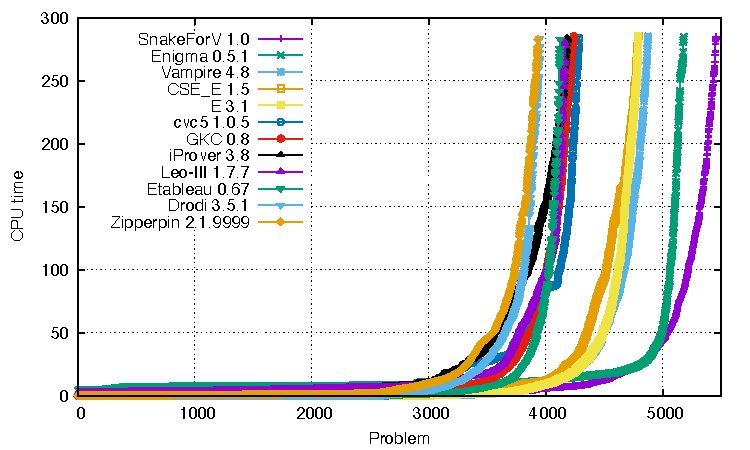
\includegraphics[width=0.6\textwidth]{FOF_THM_RFO_PPP.pdf}
\vspace*{-1em}
\caption{CPU times for {\tt FOF\_THM\_RFO\_*}}
\label{PPPPlot}
\end{figure}

%--------------------------------------------------------------------------------------------------
\section{The SZS Ontologies}
\label{SZS}

The SZS ontologies~\cite{Sut08-KEAPPA} (named ``SZS'' after the authors of the first presentation 
of the ontologies~\cite{SZS03}) provide values to specify the logical status of problems and
solutions, and to describe logical data.
The Success ontology provides values for the logical status of a conjecture ``C'' with respect to a 
set of axioms ``Ax'', e.g., a TPTP problem whose conjecture is a logical consequence of the axioms 
is tagged as a {\tt Theorem} (as in Figure~\ref{ExampleHeader}), and a model finder that 
establishes that a set of axioms (with no conjecture) is consistent should report 
{\tt Satisfiable}.
The Success ontology is also used to specify the semantic relationship between the parents ``Ax''
and inferred formulae ``C'' of an inference, as done in the TPTP format for derivations (see 
Section~\ref{TSTP}).
The NoSuccess ontology provides reasons why an ATP system/tool has failed, e.g., an ATP system 
might report {\tt Timeout}.
The Dataform ontology provides values for describing the form of logical data, as might be output 
from an ATP system/tool, e.g., a model finder might output a {\tt FiniteModel}.
Figure~\ref{SZSExtract} shows some of the salient nodes of the ontologies.
Their expanded names and their (abbreviated) definitions are listed in Figure~\ref{SZSTable}.

\begin{figure}[htb]
\centering
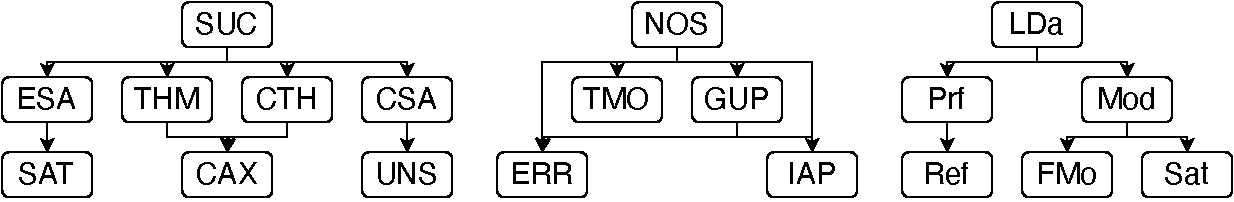
\includegraphics[width=0.75\textwidth]{SZSExtract.pdf}
\caption{Extract of the SZS ontologies}
\label{SZSExtract}
\end{figure} 

\begin{figure}[htb]
\centering
\begin{tabular}{lll}
\hline
{\tt SUC} & {\tt Success}             & 
The logical data has been processed successfully. \\
{\tt ESA} & {\tt Equisatisfiable}     & 
There exists a model of Ax iff there exists a model of C.\\
{\tt SAT} & {\tt Satisfiable}         & 
Some interpretations are models of Ax.\\
{\tt THM} & {\tt Theorem}             & 
All models of Ax are models of C.\\
{\tt CTH} & {\tt CounterTheorem}      & 
All models of Ax are models of ~C.\\
{\tt CAX} & {\tt ContradictoryAxioms} & 
No interpretations are models of Ax.\\
{\tt CSA} & {\tt CounterSatisfiable}  & 
Some models of Ax are models of {\raisebox{0.4ex}{\texttildelow}}C.\\
{\tt UNS} & {\tt Unsatisfiable}       & 
All interpretations are models of {\raisebox{0.4ex}{\texttildelow}}Ax.\\
\hline
{\tt NOS} & {\tt NoSuccess}           & 
The logical data has not been processed successfully. \\
{\tt ERR} & {\tt Error}               & 
Stopped due to an error. \\
{\tt TMO} & {\tt Timeout}             & 
Stopped because a time limit ran out. \\
{\tt GUP} & {\tt GaveUp}              & 
Gave up of its own accord. \\
{\tt IAP} & {\tt Inappropriate}       & 
Gave up because it cannot process this type of data. \\
\hline
{\tt LDa} & {\tt LogicalData}         & 
Logical data. \\
{\tt Prf} & {\tt Proof}               & 
A proof. \\
{\tt Ref} & {\tt Refutation}          & 
A refutation (ending with $false$). \\
{\tt Mod} & {\tt Model}               & 
A model. \\
{\tt FMo} & {\tt FiniteModel}         & 
A model with a finite domain. \\
{\tt Sat} & {\tt Saturation}          & 
A saturated set of formulae. \\
\hline
\end{tabular}
\caption{SZS ontology values}
\label{SZSTable}
\end{figure} 

The SZS standard also specifies the precise way in which the ontology values should be presented
in ATP system output, in order to facilitate easy processing.
For example, if an ATP system has established that a conjecture is not a theorem of the axioms,
by finding a finite countermodel of the axioms and negated conjecture, the SZS format output 
would be (see Section~\ref{TSTP} for the format of the annotated formulae)~\ldots \\
\begin{minipage}{\textwidth}
\begin{verbatim}
    % SZS status CounterSatisfiable
    % SZS output start FiniteModel
    ... annotated formulae for the finite model 
    % SZS output end FiniteModel
\end{verbatim}
\end{minipage}

\vspace*{1em}

%--------------------------------------------------------------------------------------------------
\section{Specialist Problem Classes}
\label{SPCs}

The problems in the TPTP problem library are divided into Specialist Problem Classes (SPCs) -- 
classes of problems with the same recognizable logical, language, and syntactic characteristics.
% SPCs added in v4.1.0 15/06/10
Evaluation of ATP systems within SPCs makes it possible to say which systems work well for what 
types of problems. 
The appropriate level of subdivision for SPCs is that at which less subdivision would merge 
SPCs for which ATP systems have distinguishable behaviour, and at which further subdivision
would unnecessarily split SPCs for which ATP systems have reasonably homogeneous behaviour.
Empirically, homogeneity is ensured by examining the patterns of system performance across the 
problems in each SPC. 
For example, the separation of ``essentially propositional'' problems was motivated by observing 
that SPASS~\cite{WA+99} performed differently on the ALC problems in the SYN domain of the TPTP.
A data-driven test of homogeneity is also possible~\cite{FS02}.

The characteristics currently used to define the SPCs in the TPTP are shown in 
Figure~\ref{SPCCharacteristics}.
Using these characteristics 223 SPCs are defined in TPTP v8.2.0. 
For example, the SPC
% Some examples are:
% {\tt CNF\_SAT\_EPR\_PEQ\_UEQ} -- clause normal form satisfiable clauses that are effectively
% propositional, have purely equality literals in unit equality clauses;
% {\tt FOF\_THM\_RFO\_SEQ} -- first-order theorems that are ``really first-order'' (not known
% to be effectively propositional), and contain some (not only) equality;
{\tt TF0\_THM\_NEQ\_ARI} contains typed monomorphic first-order theorems that have no equality but 
include arithmetic.
The header section of each problem in the TPTP problem library (see Section~\ref{TPTP}) includes 
its SPC.
The SPCs are used when computing the TPTP problems difficulty ratings (see Section~\ref{Ratings}).

\begin{figure}[bht]
\centering
\begin{packed_itemize}
\item TPTP language: \\
      \begin{tabular}{@{}p{5cm}l}
      {\tt CNF} -- Clause Normal Form &
      {\tt FOF} -- First-Order Form \\
      {\tt TF0/1} -- Typed First-order & Monomorphic/Polymorphic \\
      {\tt TX0/1} -- Typed eXtended f-o & Monomorphic/Polymorphic \\
      {\tt TH0/1} -- Typed Higher-order & Monomorphic/Polymorphic \\
      {\tt NX0/1} -- Non-classical {\tt TX0/1} &
      {\tt NH0/1} -- Non-classical {\tt TH0/1} \\
      \end{tabular}
\item SZS status: \\
      \begin{tabular}{@{}p{5cm}l}
      {\tt THM} -- Theorem &
      {\tt CSA} -- CounterSAtisfiable \\
      {\tt CAX} -- Contradictory AXioms & \\
      {\tt UNS} -- UNSatisfiable &
      {\tt SAT} -- SATisfiable \\
      {\tt UNK} -- UNKown &
      {\tt OPN} -- OPeN \\
      \end{tabular}
\item Order (for {\tt CNF} and {\tt FOF}): \\
      {\tt PRP} -- PRoPositional \\
      {\tt EPR} -- Effectively PRopositional (known to be reducible to {\tt PRP}) \\
      {\tt RFO} -- Real First-Order (not known to be reducible to {\tt PRP})
\item Equality: \\
      \begin{tabular}{@{}p{5cm}l}
      {\tt NEQ} -- No EQuality &
      {\tt EQU} -- EQUality (some or pure) \\
      {\tt SEQ} -- Some (not pure) EQuality &
      {\tt PEQ} -- Pure EQuality \\
      {\tt UEQ} -- Unit EQuality {\tt CNF} &
      {\tt NUE} -- Non-Unit Equality {\tt CNF} \\
      \end{tabular}
\item Hornness (for {\tt CNF}): \\
      \begin{tabular}{@{}p{5cm}l}
      {\tt HRN} -- HoRN &
      {\tt NHN} -- Non-HorN
      \end{tabular}
\item Arithmetic (for {\tt T*} languages): \\
      \begin{tabular}{@{}p{5cm}l}
      {\tt ARI} -- ARIthmetic &
      {\tt NAR} -- No ARithmetic
      \end{tabular}
\end{packed_itemize}
\caption{SPC characteristics}
\label{SPCCharacteristics}
\end{figure} 

%--------------------------------------------------------------------------------------------------
\section{Problem Difficulty Ratings}
\label{Ratings}

Each TPTP problem has a difficulty rating that provides a well-defined measure of how difficult 
the problem is for current ATP systems~\cite{SS01}.
The ratings are based on performance data in the TSTP (see Section~\ref{TSTP}), and are updated
in each TPTP edition.
The TPTP tags problems that are designed specifically to be suited or ill-suited to some ATP
system, calculus, or control strategy as {\em biased}
(this includes the {\tt SYN000} problems, which are designed for testing ATP systems' parsers).
The biased problems are excluded from the calculations.
Rating is then done separately for each SPC.

First, a partial order between systems is determined according to whether or not a system 
solves a strict superset of the problems solved by another system. 
If a strict superset is solved, the first system is said to {\em subsume} the second. 
The union of the problems solved by the non-subsumed systems defines the state-of-the-art -- all 
the problems that are solved by any system. 
The fraction of non-subsumed systems that fail on a problem is the difficulty rating 
for the problem:
problems that are solved by all of the non-subsumed systems get a rating of 0.00 (``easy'');
problems that are solved by some of the non-subsumed systems get a rating between 
0.00 and 1.00 (``difficult''); 
problems that are solved by none of the non-subsumed systems get a rating of 1.00 (``unsolved'').
As additional output, the systems are given a rating for each SPC -- the fraction of difficult 
problems they can solve.

The TPTP difficulty ratings provide a way to assess progress in the field -- as problem that 
are unchanged are not actually getting easier, decreases in their difficulty ratings are evidence 
of progress in ATP systems.
Figures~\ref{Ratings_v5.0.0_v6.4.0} and~\ref{Ratings_v6.3.0_v8.2.0} plot the average difficulty
ratings overall and for each of the four language forms in the TPTP World (after some sensible
data cleaning).
Figure~\ref{Ratings_v5.0.0_v6.4.0} is taken from~\cite{Sut17}, published in 2017.
It plots the average ratings for the 14527 problems that had been unchanged and whose ratings 
had not been stuck at 0.00 or 1.00, from v5.0.0 that was released in 2010 to v6.4.0 that was
released in 2016. 
Figure~\ref{Ratings_v6.3.0_v8.2.0} is taken from~\cite{SK+24}, published in 2024.
It plots the average ratings for the 16236 problems that had been unchanged and whose ratings 
had not been stuck at 0.00 or 1.00, from v6.3.0 that was released in 2016 to v8.2.0 that was
released in 2023. 
The two figures’ plots dovetail quite well, which gives confidence that they really are 
comparable (there are some minor differences caused by slightly different different data cleaning 
and by recent refinements to the difficulty rating calculations). 
The older plots show a quite clear downward trend both overall and for the four language forms, 
while the new plots do not. 
Possible reasons are discussed in~\cite{SK+24}.

\begin{figure}[t!]
\centering
\begin{minipage}[t]{.49\textwidth}
  \centering
  \includegraphics[width=\textwidth]{RatingsDecline_v5.0.0_v6.4.0.pdf}
  \vspace*{-2em}
  \caption{Ratings from v5.0.0 to v6.4.0}
  \label{Ratings_v5.0.0_v6.4.0}
\end{minipage}
\begin{minipage}[t]{.49\textwidth}
  \centering
  \includegraphics[width=\textwidth]{RatingsDecline_v6.3.0_v8.2.0.pdf}
  \vspace*{-2em}
  \caption{Ratings from v6.3.0 to v8.2.0}
  \label{Ratings_v6.3.0_v8.2.0}
\end{minipage}
\end{figure}


%--------------------------------------------------------------------------------------------------
\section{SystemOnTPTP and StarExec}
\label{StarExec}

Some of the early users of the TPTP problem library (see Section~\ref{TPTP}) were working in
disciplines other than computer science, e.g. (with a few exemplar references), in mathematics 
\cite{Qua92-Book,MP96}, logic~\cite{GO86,Jec95}, management~\cite{PB+92-TR,PM94}, planning 
\cite{SE94}, etc. 
These users often selected the Otter ATP system~\cite{McC03-Otter} for their experiments, as
it was readily available and easy enough to install. 
As the TPTP World evolved it was clear that more powerful ATP systems were available, especially 
evident in the CADE ATP System Competition (see Section~\ref{CASC}).
However, these more powerful systems were often not as easy to obtain and install.
In order to make use of ATP easier for non-geek users, an NSF grant was obtained\footnote{%
NSF Award 1405674} to build the SystemOnTPTP online service, which provides hardware and a web 
interface for users to submit their problems to most recent versions of a wide range of ATP 
systems.
SystemOnTPTP also provides recommendations for ATP systems that might be most likely to solve
a problem, based on the SPC of the user's problem and the system ratings for the SPC
(see Sections~\ref{SPCs} and~\ref{Ratings}). 
SystemOnTPTP can run ATP systems (e.g., the recommended systems) in competition
parallel~\cite{SS99-FLAIRS}.
The core SystemOnTPTP service is supported by the SystemB4TPTP service that provides tools to
prepare problems for submission to ATP systems, e.g., axiom selection~\cite{HV11}, a scripting
language~\cite{Sut14}, type checking~\cite{KSR16}, and the SystemOnTSTP service that provides 
tools for analysing solutions output from SystemOnTPTP, 
e.g., identification of interesting lemmas in a proof~\cite{PGS06}, proof checking~\cite{Sut06},
interactive viewing of derivations~\cite{TPS07}.
The web page 
\href{https://www.tptp.org/cgi-bin/SystemOnTPTP}{{\tt www.tptp.org/cgi-bin/SystemOnTPTP}} 
provides the entry point to web pages for interactive use of the services.
While many users enjoy interactive browser-based usage, it is also easy to use the services 
programmatically; in fact this is where most of the use comes from.
In 2023 there were 887287 requests serviced (an average of one every 36 seconds), from 286 
countries.
One heavy programmatic user is the Sledgehammer component of the interactive theorem prover
Isabelle~\cite{PB10}.

The TPTP problem library was motivated (see Section~\ref{TPTP}) by the need to provide support
for meaningful ATP system evaluation.
This need was (or became) evident in other logic solver communities, e.g., SAT~\cite{HS00-SATLIB} 
and SMT~\cite{BST10}.
For many years testing of logic solvers was done on individual developer's computers. 
In 2010 a proposal for centralised hardware and software support was developed,
and in 2011 a \$2.11 million NSF grant\footnote{%
NSF Awards 1058748 and 1058925, led by Aaron Stump and Cesare Tinelli at the University of Iowa} 
was obtained.
This grant led to the development and availability of StarExec Iowa~\cite{SST14} in 2012,
and a subsequent \$1.00 million grant\footnote{%
NSF Award 1730419} in 2017 expanded StarExec to Miami.
StarExec has been central to much progress in logic solvers over the last 10 years, supporting
16 logic solver community, used for running many of their annual competitions~\cite{BB+19},
and supporting many many users.

It has recently been announced that StarExec Iowa will be decommissioned. 
The maintainer of StarExec Iowa explained that ``the plan is to operate StarExec as usual for 
competitions Summer 2024 and Summer 2025, and then put the system into a read-only mode for one 
year (Summer 2025 to Summer 2026)''.
While StarExec Miami will continue to operate while funding is available, but it will not be able
to support the large number of logic solver communities that use the larger StarExec Iowa cluster.
Thus in the long run it will be necessary for StarExec users to transition to new environments,
and several plans are (at the time of writing) being discussed.
One effort is to containerise StarExec and ATP systems from the TPTP World, with the goal of
running in a Kubernetes framework on Amazon Web Services.
If successful, this will allow communities and individual users to run their own StarExec.

%--------------------------------------------------------------------------------------------------
\section{The CADE ATP System Competition}
\label{CASC}

The CADE ATP System Competition (CASC)~\cite{Sut16} is the annual evaluation of fully automatic,
classical logic, ATP systems - the world championship for such systems.
CASC is held at each CADE (the International Conference on Automated Deduction) and IJCAR
(the International Joint Conference on Automated Reasoning) conference -- the major forums
for the presentation of new research in all aspects of automated deduction.
One purpose of CASC is to provide a public evaluation of the relative capabilities of ATP systems.
Additionally, CASC aims to
stimulate ATP research,
motivate development and implementation of robust ATP systems that can be easily and usefully
deployed in applications,
provide an inspiring environment for personal interaction between ATP researchers,
and
expose ATP systems within and beyond the ATP community.
Over the years CASC has been a catalyst for impressive improvements in ATP, stimulating both 
theoretical and implementation advances~\cite{Nie02-Paper}.
It has provided a forum at which empirically successful implementation efforts are acknowledged 
and applauded, and at the same time provides a focused meeting at which novice and experienced 
developers exchange ideas and techniques. 
The first CASC was held at CADE-13 in 1996, at DIMACS in Rutgers University, USA.
The CASC web site provides access to all the details:
\href{http://www.tptp.org/CASC/}{{\tt www.tptp.org/CASC}}.
Of particular interest for this IJCAR is that CASC was conceived of 30 years ago in 1994 after 
CADE-12 in Nancy, when Christian Suttner and I were sitting on a bench under a tree in 
Parc~de~la~Pépinière burning time before our train departures.

CASC is run in divisions according to problem and system characteristics, in a coarse version
of the SPCs (see Section~\ref{SPCs}).
Problems for CASC are taken from the TPTP problem library (see Section~\ref{TPTP}), and some 
other sources. 
The TPTP problem ratings (see Section~\ref{Ratings}) are used to select appropriately difficult
problems from the TPTP problem library.
The systems are ranked according to the number of problems solved with an acceptable proof/model 
output.
Ties are broken according to the average time over problems solved.
In addition to the ranking criteria, three other measures are made and presented in the results:
the {\em state-of-the-art (SoTA) contribution} quantifies the unique abilities of each system;
the {\em efficiency measure} is a combined measure that balances the time taken for each problem 
solved against the number of problems solved;
the {\em core usage} is the average of the ratios of CPU time to wall clock time used, over the 
problems solved.

The design and organization of CASC has evolved over the years to a sophisticated state.
In the years from CASC-26 to CASC-J12 the competition stayed quite stable, but each year
the various divisions, evaluations, etc., were optimized (as was also the case in prior years
when step changes also peturbed the competition design).
The changes in the divisions reflect the changing demands and interest in different types
of ATP problems, and decisions made for CASC (alongside the TPTP) have had an influence on 
the directions of development in ATP.
Over the years 11 divisions have been run~\ldots
\begin{packed_itemize}
\item The Clause Normal Form (CNF) division from CASC-13 in 1996 to CASC-23 in 2011.
\item The Satisfiability (SAT) division from CASC-14 in 1997 to CASC-22 in 2009.
\item The First-order Form (FOF) division from CASC-15 in 1998 to ... ongoing.
\item The Effectively Propositional (EPR) division from CASC-JC in 2001 to CASC-27 in 2019.
\item The First-order Non-theorem (FNT) division from CASC-21 in 2007 to CASC-29 in 2023.
\item The Large Theory Batch (LTB) division from CASC-J4 in 2008 to CASC-J11 in 2022.
\item The Typed Higher-order (THF) division from CASC-J5 in 2010 to ... ongoing.
\item The Typed First-order with Arithmetic (TFA) division from CASC-23 in 2011 to ... ongoing.
\item The Typed First-order Non-theorem (TFN) division from CASC-25 in 2015 to CASC-J8 in 2016,
      revived in CASC-29 in 2003 to ... ongoing.
\item The Sledgehammer (SLH) division from CASC-26 in 2017 to ... ongoing.
\item The I Challenge You (ICU) division introduced for CASC-J12 in 2024.
\end{packed_itemize}

Over all 20 CASCs so far 111 distinct ATP systems have been entered.  
For each CASC the division winners of the previous CASC are automatically entered to provide 
benchmarks against which progress can be judged.
% Additionally, the well known Otter system was entered in every CASC from 2002 to 2011, as a 
% fixed point against which progress could be judged.
% By 2011 Otter was no longer competitive, and was replaced by Prover9 2009-11A in 2012.
% Almost all the ATP systems have come from academia, partially due to the CASC requirement that 
% source code for the systems must be published on the CASC web site (if the source cannot be made 
% public, the system must run the demonstration division).
Some systems have emerged as dominant in some of the divisions, with Vampire being a well-known
example.
The strengths of these systems stem from four main areas:
solid theoretical foundations, significant implementation efforts (in terms of coding and data 
structures), extensive testing and tuning, and an understanding of how to optimize for CASC.

%--------------------------------------------------------------------------------------------------
\section{TPTP World Users}
\label{Users}

Over the years the TPTP World has provided a platform upon which ATP users have presented their 
needs to ATP system developers, who have then adapted their ATP systems to the users’ needs.
% The TSTP is often used by ATP system developers to examine solutions to problems, and thus 
% understand how they can be solved, leading to improvements to their own systems. 
The interplay between the TPTP problem library (see Section~\ref{TPTP}) and the CADE ATP
System Competition (see Section~\ref{CASC}) has been particularly effective as a conduit for 
ATP users to provide samples of their problems to ATP system developers.
Users' problems that are contributed to the TPTP are eligible for use in CASC.
The problems are then exposed to ATP system developers, who improve their systems' performances 
on the problems, in order to perform well in CASC.
This completes a cycle that provides the users with more effective tools for solving their 
problems.

Many people have contributed to the TPTP World, with problems, software, advice, expertise,
and enthusiasm. 
I am grateful to them all, and here are just a few who have made salient contributions (ordered
rough by date of the contributions mentioned):
\begin{packed_itemize}
\item Christian Suttner - The TPTP problem library and CASC.             % 1992
\item Stephan Schulz - Technical advice                                  % 1996
\item Jeff Pelletier - Early support, advice, and problem contributions. % 2001
\item Allen van Gelder - BNF and parser                                  % 2006
\item Adam Pease and Josef Urban - Large theory problems                 % 2010
\item Christoph Benz{\"u}ller and Chad Brown - TH0                       % 2010
\item Koen Claessen and Peter Baumgartner and Stephan Schulz - TF0       % 2012
\item Jasmin Blanchette - Sledgehammer to SystemOnTPTP, TF1              % 2013
\item Andrei Paskevich - TF1                                             % 2013
\item Cezary Kaliszyk and Florian Rabe - TH1                             % 2016
\item Evgeny Kotelnikov - TXF                                            % 2018
\item Christoph Benz{\"u}ller and Alexander Steen - NTF                  % 2022
\end{packed_itemize}
Thank you!

%--------------------------------------------------------------------------------------------------
\section{Conclusion}
\label{Conclusion}

This paper 

This section has naturally focused on the successful parts of the TPTP history.
There have also been some failed developments and suboptimal (in retrospect) decisions \frownie{}.
For example, in 2015 there was an attempt to develop a description logic form for the TPTP 
language. 
While some initial progress was made, it ground to a halt without support from the description 
logic community.
A suboptimal design decision, rooted in the early days of the TPTP, is the naming scheme used for 
problem files. 
The naming scheme uses three digits to number the problems in each domain, thus setting a limit 
of 1000 problems, which failed to anticipate the numbers of problems that would be contributed 
to some of the problem domains.
This has been overcome by creating multiple domain directories where necessary, but if it were 
to be done again, six or eight digit problem numbers shared across all domains would be an 
improvement.

Currently this work is being extended to 

None of this would have happened without the early strategic insights of Christian Suttner,
with his willingness to let me do the organization without interference. 
Maybe his most wonderful contribution (which took him over two hours to produce when he
was visiting me at James Cook University -- I think he took a nap \smiley) is his 
plain-language definition of automated theorem proving: 
``the derivation of conclusions that follow inevitably from known facts''.

%--------------------------------------------------------------------------------------------------
\bibliographystyle{plain}
\bibliography{Bibliography.bib}
%--------------------------------------------------------------------------------------------------
\end{document}
%--------------------------------------------------------------------------------------------------
